\documentclass[10pt,letterpaper]{article}
\usepackage[lmargin=2.2in,rmargin=0.7in,tmargin=1.0in,bmargin=1.0in]{geometry}
\usepackage{notes}
\usetikzlibrary{positioning,arrows.meta}

\begin{document}

\begin{center}
\Large\textbf{DAY 26 -- Matrices and Linear Systems}\\
\normalsize (Section 4.1)
\end{center}

%%%%%%%%%%%%%%%%%%%%%%%%%%%%%%%%%%%%%%%%%%%%%%%%%%%%%%%%%%%%%%%%%%%%%%%%
\section{Linear Algebra}

\subsection{Goal and Motivation}
The goal for today is to learn the basics of \textbf{linear algebra} — math involving \textit{matrices} and \textit{vectors}. We will use linear algebra to analyze systems of
differential equations. We begin with the tools
for solving algebraic linear systems such as
\[
\begin{dcases}
-3x+y=-1,\\
-2x+y=1.
\end{dcases}
\]
The objective of this problem is to find two numbers $x$ and $y$. In linear algebra, we think of this problem as finding the one unknown \textit{vector}
$$
    \textbf{x} = \begin{pmatrix}
        x\\y
    \end{pmatrix}.
$$

\subsection{Vectors and Matrices}
A 2D \textbf{vector} is a two-by-one arrangement of numbers grouped together as one object:
$$
    \textbf{v} = \begin{pmatrix}
        a\\b
    \end{pmatrix}
$$
The numbers $a$ and $b$ are called \textbf{components} of $\textbf{v}$.
I may occasionally use the Calculus III notation $\textbf{v}=\cvec{a,b}$. The textbook uses the notation $\textbf{v}=(a,b)$. They all mean the same thing. You may think of \textbf{v} as a point in two-dimensional space.

A 2D \textbf{matrix} is a two-by-two arrangement of numbers
\[
A=
\begin{pmatrix}
a & b\\
c & d
\end{pmatrix}.
\]
The convention is to use bold-face lower-case letters for vectors (like \textbf{x}, \textbf{b}, \textbf{u}, \textbf{v}) and capital letters for matrices (like $A$, $B$, $I$). But when you are hand-writing vectors, people typically use an over-head arrow or an underline
$$
    \textbf{v} = \vec{v} = \underline{v}.
$$
Matrices and vectors can generally contain many more components, but in this class, we restrict our study to $2\times 2$ and $2\times 1$.

%-------------------------------------------------------------

\subsection{Geometric Interpretation}

How many solutions does the linear system
\[
\begin{dcases}
ax+by=f,\\
cx+dy=g
\end{dcases}
\]
have? Each equation describes a line in the $xy$-plane.
A solution $(x,y)$ must lie on both lines, so solving
the system means finding their intersection.

There are three possibilities:
\begin{enumerate}
    \item The lines intersect once: \textbf{one solution}.
    \item The lines are distinct and parallel:
    \textbf{no solution}.
    \item The lines coincide:
    \textbf{infinitely many solutions}.
\end{enumerate}
Sketching the lines helps us determine which case we have.

\begin{example}[1]{
For each pair of lines, sketch them and find the
intersection, if any.
\begin{enumerate}
    \item[(a)] $y=3x-1,\qquad y=2x+1$.
    \item[(b)] $y=4x+1,\qquad y=4x-1$.
    \item[(c)] $y=x+2,\qquad 2y=2x+4$.
\end{enumerate}
}

\paragraph{(a)}
Set the two expressions for $y$ equal:
\[
3x-1=2x+1
\implies x=2.
\]
Substituting gives $y=5$, so the intersection is
\[
\boxed{(x,y)=(2,5).}
\]

\begin{center}
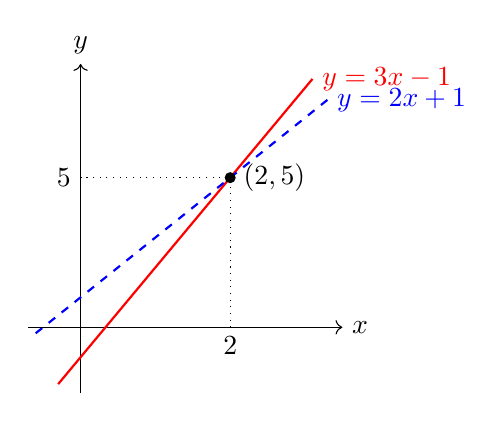
\begin{tikzpicture}[x=0.95cm,y=0.38cm]
    % Axes
    \draw[->] (-0.7,0) -- (3.5,0) node[right] {$x$};
    \draw[->] (0,-2.2) -- (0,8.8) node[above] {$y$};

    % Lines
    \draw[red,thick,domain=-0.3:3.1]
        plot (\x,{3*\x-1});
    \draw[blue,dashed,thick,domain=-0.6:3.3]
        plot (\x,{2*\x+1});

    % Intersection and guides
    \draw[dotted] (2,0) -- (2,5) -- (0,5);
    \fill (2,5) circle (2pt);
    \node[right] at (2.05,5) {$(2,5)$};
    \node[below] at (2,0) {$2$};
    \node[left] at (0,5) {$5$};

    % Labels
    \node[red,right] at (3.1,8.3) {$y=3x-1$};
    \node[blue,right] at (3.3,7.6) {$y=2x+1$};
\end{tikzpicture}
\end{center}

\paragraph{(b)}
The lines have the same slope but different intercepts.
They are \textbf{parallel}, so there is no intersection.

\begin{center}
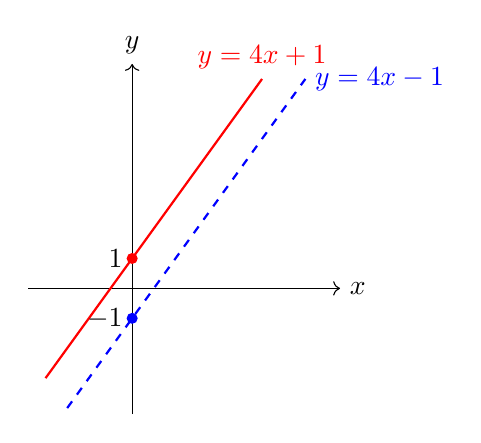
\begin{tikzpicture}[x=1.1cm,y=0.38cm]
    % Axes
    \draw[->] (-1.2,0) -- (2.4,0) node[right] {$x$};
    \draw[->] (0,-4.2) -- (0,7.5) node[above] {$y$};

    % Lines
    \draw[red,thick,domain=-1:1.5]
        plot (\x,{4*\x+1});
    \draw[blue,dashed,thick,domain=-0.75:2]
        plot (\x,{4*\x-1});

    % Intercepts
    \fill[red] (0,1) circle (2pt);
    \fill[blue] (0,-1) circle (2pt);
    \node[left] at (0,1) {$1$};
    \node[left] at (0,-1) {$-1$};

    % Labels
    \node[red,above] at (1.5,7) {$y=4x+1$};
    \node[blue,right] at (2,7) {$y=4x-1$};
\end{tikzpicture}
\end{center}

\paragraph{(c)}
Dividing the second equation by $2$ gives $y=x+2$.
The lines are \textbf{coincident}, so there are
infinitely many intersections. Every point on
$y=x+2$ solves both equations.

\begin{center}
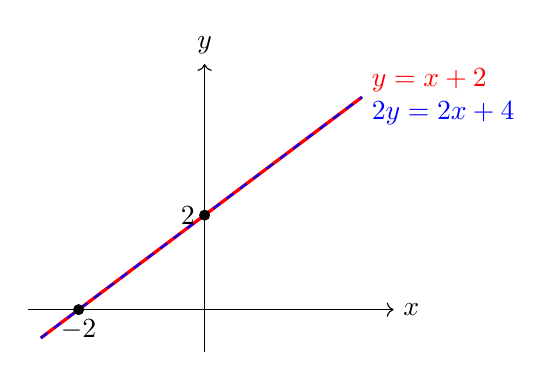
\begin{tikzpicture}[x=0.8cm,y=0.6cm]
    % Axes
    \draw[->] (-2.8,0) -- (3,0) node[right] {$x$};
    \draw[->] (0,-0.9) -- (0,5.2) node[above] {$y$};

    % Coincident lines: draw one over the other
    \draw[red,very thick] (-2.6,-0.6) -- (2.5,4.5);
    \draw[blue,dashed,thick] (-2.6,-0.6) -- (2.5,4.5);

    % Intercepts
    \fill (-2,0) circle (2pt);
    \fill (0,2) circle (2pt);
    \node[below] at (-2,0) {$-2$};
    \node[left] at (0,2) {$2$};

    % Labels
    \node[align=left,right] at (2.5,4.5)
        {\textcolor{red}{$y=x+2$}\\
         \textcolor{blue}{$2y=2x+4$}};
\end{tikzpicture}
\end{center}
\end{example}


%%%%%%%%%%%%%%%%%%%%%%%%%%%%%%%%%%%%%%%%%%%%%%%%%%%%%%%%%%%%%%%%%%%%%%%%
\section{Linear Algebra Operations}
Before going further into linear systems, let's back up and learn some arithmetic operations. 

\subsection{Addition}

You may add two vectors: 
\[
\textbf{u}+\textbf{v}=
\begin{pmatrix}
u_1\\u_2
\end{pmatrix}
+
\begin{pmatrix}
v_1\\v_2
\end{pmatrix}
=
\begin{pmatrix}
u_1+v_1\\u_2+v_2.
\end{pmatrix}
\]
For example,
\[
\begin{pmatrix}1\\3\end{pmatrix}
+
\begin{pmatrix}4\\-2\end{pmatrix} = 
\begin{pmatrix}4+1\\3-2\end{pmatrix} = 
\begin{pmatrix}5\\1\end{pmatrix}.
\]
You can also add two matrices. The common rule is to add component-by-component. You cannot add a vector to a matrix because they have different sizes. Subtraction works the same way.

\begin{example}[2]{
Compute $A+B$ and $A-B$, where
\[
A=
\begin{pmatrix}
1&4\\
-2&3
\end{pmatrix},
\qquad
B=
\begin{pmatrix}
2&-1\\
5&3
\end{pmatrix}.
\]
}
Adding corresponding entries gives
\[
A+B=
\begin{pmatrix}
1+2&4-1\\
-2+5&3+3
\end{pmatrix}
=
\boxed{
\begin{pmatrix}
3&3\\
3&6
\end{pmatrix}.
}
\]
Subtracting corresponding entries gives
\[
A-B=
\begin{pmatrix}
1-2&4-(-1)\\
-2-5&3-3
\end{pmatrix}
=
\boxed{
\begin{pmatrix}
-1&5\\
-7&0
\end{pmatrix}.
}
\]
\end{example}
%-------------------------------------------------------------
\subsection{Scalar Multiplication}

A \textbf{scalar} is a number. We will generally use
lower-case Greek letters for scalars (like
$\alpha$, $\beta$, $\lambda$).
Multiplying a vector by a scalar multiplies every component:
\[
\alpha\mathbf{v}
=
\alpha
\begin{pmatrix}
v_1\\v_2
\end{pmatrix}
=
\begin{pmatrix}
\alpha v_1\\\alpha v_2
\end{pmatrix}.
\]
For example,
\[
2\begin{pmatrix}1\\3\end{pmatrix}
=
\begin{pmatrix}2\\6\end{pmatrix}.
\]
Multiplying a matrix by a scalar works the same way:
multiply every entry by the scalar.

\begin{example}[3]{
Compute $\lambda A$, where
\[
\lambda=-2,
\qquad
A=
\begin{pmatrix}
1&4\\
-2&3
\end{pmatrix}.
\]
}
Multiply every entry by $-2$:
\[
\lambda A
=
\begin{pmatrix}
(-2)(1)&(-2)(4)\\
(-2)(-2)&(-2)(3)
\end{pmatrix}
=
\boxed{
\begin{pmatrix}
-2&-8\\
4&-6
\end{pmatrix}.
}
\]
\end{example}

%-------------------------------------------------------------
\subsection{Matrix-Vector Multiplication}

The basic calculation is to multiply a row by a column:
multiply corresponding entries, then add.
\[
\begin{pmatrix}a&b\end{pmatrix}
\begin{pmatrix}x\\y\end{pmatrix}
=ax+by.
\]
This calculation is called a \textbf{dot product}.
The result is a scalar. For example,
\[
\begin{pmatrix}1&3\end{pmatrix}
\begin{pmatrix}4\\-2\end{pmatrix}
=1(4)+3(-2)=-2.
\]
To multiply a matrix by a vector, repeat this
calculation for each row:
\[
A\mathbf{x}
=
\begin{pmatrix}
a&b\\
c&d
\end{pmatrix}
\begin{pmatrix}
x\\y
\end{pmatrix}
=
\begin{pmatrix}
ax+by\\
cx+dy
\end{pmatrix}.
\]
The first row produces the first component;
the second row produces the second component.
Thus, the result is a vector. \textbf{Key Idea}: matrix-vector multiplication is just doing two dot products.

\begin{example}[4]{
Compute
\[
\begin{pmatrix}
1&4\\
-2&3
\end{pmatrix}
\begin{pmatrix}2\\1\end{pmatrix}.
\]
}
Multiply each row by the column:
\[
\begin{pmatrix}
1&4\\
-2&3
\end{pmatrix}
\begin{pmatrix}2\\1\end{pmatrix}
=
\begin{pmatrix}
1(2)+4(1)\\
-2(2)+3(1)
\end{pmatrix}
=
\boxed{
\begin{pmatrix}6\\-1\end{pmatrix}.
}
\]
\end{example}

%-------------------------------------------------------------
\subsection{Matrix-Matrix Multiplication}

Multiplying two $2\times2$ matrices means computing
\textbf{four dot products}, one for each entry of
the result:
\[
AB=
\begin{pmatrix}
a&b\\
c&d
\end{pmatrix}
\begin{pmatrix}
e&f\\
g&h
\end{pmatrix}
=
\begin{pmatrix}
ae+bg&af+bh\\
ce+dg&cf+dh
\end{pmatrix}.
\]
Each entry comes from a dot product between a \textbf{row of A}
and a \textbf{column of B}:
\[
\red{A}\blue{B}=
\begin{pmatrix}
\red{\text{row 1}}\cdot\blue{\text{column 1}}&
\red{\text{row 1}}\cdot\blue{\text{column 2}}\\
\red{\text{row 2}}\cdot\blue{\text{column 1}}&
\red{\text{row 2}}\cdot\blue{\text{column 2}}
\end{pmatrix}.
\]
\begin{example}[5]{
Compute
\[
\begin{pmatrix}
1&2\\
3&4
\end{pmatrix}
\begin{pmatrix}
2&0\\
1&5
\end{pmatrix}.
\]
}
Compute the four dot products:
\begin{align*}
\text{Top left:}\quad
&\begin{pmatrix}1&2\end{pmatrix}
\begin{pmatrix}2\\1\end{pmatrix}=1(2)+2(1)=4,\\
\text{Top right:}\quad
&\begin{pmatrix}1&2\end{pmatrix}
\begin{pmatrix}0\\5\end{pmatrix}=1(0)+2(5)=10,\\
\text{Bottom left:}\quad
&\begin{pmatrix}3&4\end{pmatrix}
\begin{pmatrix}2\\1\end{pmatrix}=3(2)+4(1)=10,\\
\text{Bottom right:}\quad
&\begin{pmatrix}3&4\end{pmatrix}
\begin{pmatrix}0\\5\end{pmatrix}=3(0)+4(5)=20.
\end{align*}
Place each result in its corresponding position:
\[
\boxed{
AB=
\begin{pmatrix}
4&10\\
10&20
\end{pmatrix}.
}
\]
\end{example}

The order matters: in general, $AB\ne BA$.
Matrix multiplication uses row-by-column dot products,
not entry-by-entry multiplication.

%%%%%%%%%%%%%%%%%%%%%%%%%%%%%%%%%%%%%%%%%%%%%%%%%%%%%%%%%%%%%%%%%%%%%%%%
\section{Solving Linear Systems}

\subsection{Rewriting a System in Matrix Form}

Let's return to our main objective. We want to solve this system
\begin{equation}    
\begin{dcases}
ax+by=f,\\
cx+dy=g.
\end{dcases}\label{expanded}
\end{equation}
By the definition of matrix-vector multiplication,
we can write these two equations as one vector equation:
\[
\underbrace{
\begin{pmatrix}
a&b\\
c&d
\end{pmatrix}}_{A}
\underbrace{
\begin{pmatrix}x\\y\end{pmatrix}}_{\mathbf{x}}
=
\underbrace{
\begin{pmatrix}f\\g\end{pmatrix}}_{\mathbf{b}}.
\]
This means the system we want to solve can be written compactly as
\begin{equation}\label{matrix}
A\mathbf{x}=\mathbf{b}.
\end{equation}
Let's call \eqref{expanded} the \textit{expanded form} and \eqref{matrix} the \textit{matrix form}. The objective is to find the vector $\textbf{x}$, given $A$ and $\textbf{b}$.

Suppose we replace $A$, $\textbf{x}$, and $\textbf{b}$ with scalars. Then how would you solve for $x$? You can multiply both sides by the reciprocal of $A$, $A^{-1}$: 
\begin{align*}
    Ax&=b\\
    A^{-1}Ax&=A^{-1}b\\
    (1)x&=A^{-1}b\\
    x &= A^{-1}b
\end{align*}
We have similar operations for matrices. There are matrix versions of $A^{-1}$ and $(1)$.

%-------------------------------------------------------------
\subsection{Identity Matrix}

Before defining a matrix reciprocal, we need a matrix that plays the role of the number $1$. The \textbf{identity matrix}, denoted by $I$, is defined to be 
\[
I=
\begin{pmatrix}
1&0\\
0&1
\end{pmatrix}.
\]
Multiplying by $I$ leaves a vector unchanged:
\[
I\mathbf{x}
=
\begin{pmatrix}
1&0\\
0&1
\end{pmatrix}
\begin{pmatrix}x\\y\end{pmatrix}
=
\begin{pmatrix}x\\y\end{pmatrix}
=\mathbf{x}.
\]
The same holds for matrices:
\[
IA=AI=A.
\]

%-------------------------------------------------------------
\subsection{Matrix Inverse}

The matrix version of a reciprocal is called an
\textbf{inverse}. For a square matrix $A$, its inverse
$A^{-1}$ satisfies
\[
A^{-1}A=AA^{-1}=I.
\]
Thus, multiplying by $A^{-1}$ undoes multiplication
by $A$. There is a formula for the matrix inverse. If
\[
A=\begin{pmatrix}a&b\\c&d\end{pmatrix}
\]
then the inverse is given by
\[
\boxed{
A^{-1}
=\frac{1}{ad-bc}
\begin{pmatrix}
d&-b\\
-c&a
\end{pmatrix},
}
\]
provided that $ad-bc \neq 0$.


%-------------------------------------------------------------
\subsection{Solving the System}

Once the matrix $A^{-1}$ is calculated, we can solve the linear system by multiplication. Start with $A\textbf{x}=\textbf{b}$ and multiply both sides by $A^{-1}$:
\begin{align*}
A\mathbf{x}&=\mathbf{b},\\
A^{-1}A\mathbf{x}&=A^{-1}\mathbf{b},\\
I\mathbf{x}&=A^{-1}\mathbf{b}.
\end{align*}
Therefore, the solution to $A\textbf{x}=\textbf{b}$ is 
\[
\boxed{\mathbf{x}=A^{-1}\mathbf{b}.}
\]
Let's do an example to demonstrate how this works.

\begin{example}[6]{
Find the solution to
\[
\begin{dcases}
-3x+y=-1,\\
-2x+y=1.
\end{dcases}
\]
}
\paragraph{Step 1. Write the matrix equation.}
\[
\underbrace{
\begin{pmatrix}
-3&1\\
-2&1
\end{pmatrix}}_{A}
\underbrace{
\begin{pmatrix}x\\y\end{pmatrix}}_{\mathbf{x}}
=
\underbrace{
\begin{pmatrix}-1\\1\end{pmatrix}}_{\mathbf{b}}.
\]

\paragraph{Step 2. Find the inverse.}
We calculate the inverse using the formula
\[
A^{-1}
=\frac{1}{ad-bc}
\begin{pmatrix}
d&-b\\
-c&a
\end{pmatrix}
=\frac{1}{-1}
\begin{pmatrix}
1&-1\\
2&-3
\end{pmatrix}
=
\begin{pmatrix}
-1&1\\
-2&3
\end{pmatrix}.
\]

\paragraph{Step 3. Multiply by the right-hand side.}
\[
\mathbf{x}=A^{-1}\mathbf{b}
=
\begin{pmatrix}
-1&1\\
-2&3
\end{pmatrix}
\begin{pmatrix}-1\\1\end{pmatrix}
=
\begin{pmatrix}
(-1)(-1)+1(1)\\
(-2)(-1)+3(1)
\end{pmatrix}
=
\boxed{
\begin{pmatrix}2\\5\end{pmatrix}.
}
\]
Thus, the lines intersect at $(2,5)$, agreeing
with our earlier calculation.
\end{example}

%-------------------------------------------------------------
\subsection{Determinant}

Not every matrix has an inverse. A matrix with an inverse is called \textbf{invertible} or
\textbf{nonsingular}. A matrix without an inverse is called \textbf{singular}. There is a check to determine whether $A$ is invertible or not.

For the matrix $A$, we define its \textbf{determinant}, $\det(A)$, to be
\[
\boxed{
\det(A)=
\begin{vmatrix}\red{a}&\blue{b}\\\blue{c}&\red{d}\end{vmatrix}
=\red{ad}-\blue{bc}.
}
\]
Multiply the diagonal entries, then subtract the
product of the off-diagonal entries. 

Notice that $\det(A)$ is the denominator term in the formula for $A^{-1}$. You can determine whether $A$ is invertible based on the value of its determinant. If $\det(A)\ne0$, then $A$ is invertible. If $\det(A)=0$ then $A^{-1}$ does not exist.


\begin{example}[7]{
Determine if the following matrices are invertible.
\[
A=
\begin{pmatrix}
1&4\\
-2&3
\end{pmatrix},
\qquad
B=
\begin{pmatrix}
2&4\\
4&8
\end{pmatrix}.
\]
}
Using the formula,
\[
\det(A)=1(3)-4(-2)=11.
\]
Since $\det(A)\ne0$, we conclude that \boxed{A \text{ is invertible}}. In contrast,
\[
\det(B)=2(8)-4(4)=0,
\]
so we conclude that \boxed{B \text{ is not invertible}}.
\end{example}

%%%%%%%%%%%%%%%%%%%%%%%%%%%%%%%%%%%%%%%%%%%%%%%%%%%%%%%%%%%%%%%%%%%%%%%%
\section{Finding All Solutions}

\subsection{The Determinant Test}
Suppose you are tasked with finding \textit{all} solutions to 
$$
    \begin{pmatrix}
        a & b\\c & d
    \end{pmatrix}\textbf{x} = \begin{pmatrix}
        f \\g
    \end{pmatrix}.
$$
Recall that a linear system can have one solution, no solution, or infinitely many solutions. Begin by checking if the determinant is non-zero:
\[
\det(A)\ne0
\quad\implies\quad
\boxed{\text{one solution }\mathbf{x}=A^{-1}\mathbf{b}.}
\]
Geometrically, the two lines intersect at one point. We have already done this in Example 6.

If $\det(A)=0$, the inverse does not exist.
However, no inverse does not mean no solution.
It means we cannot use the inverse formula.
The system may have no solution or infinitely many
solutions. We must examine the equations to decide.
A system is \textbf{consistent} if it has at least
one solution and \textbf{inconsistent} if it has none.

%-------------------------------------------------------------
\subsection{When the Determinant Is Zero}

We will compare two systems with the same coefficient
matrix but different right-hand sides. Both matrices
are singular, but the systems have different numbers
of solutions. If $\det(A)=0$, then you must rewrite the system back in \textit{expanded form}, and then check whether the equations match.

\begin{example}[8]{
Find all solutions:
\[
\begin{pmatrix}
1&2\\
2&4
\end{pmatrix}
\mathbf{x}
=
\begin{pmatrix}3\\6\end{pmatrix}.
\]
}
\paragraph{Step 1. Check the determinant.}
\[
\det(A)=1(4)-2(2)=0.
\]
The matrix is singular, so we cannot use
$A^{-1}\mathbf{b}$.

\paragraph{Step 2. Compare the equations.}
Rewriting the system back in expanded form gives
\[
\begin{dcases}
x+2y=3,\\
2x+4y=6.
\end{dcases}
\]
The second equation is twice the first.
Thus, both equations describe the same line.
Every point on
\[
\boxed{x+2y=3}
\]
solves the system. There are infinitely many solutions.

\paragraph{Step 3. Solve for $y$.} If $x+2y=3$ then $y=-\tfrac{1}{2}x+\tfrac{3}{2}$. There is no restriction on $x$. Therefore, solution is all points on the line
\[
\boxed{
y=-\frac{1}{2}x+\frac{3}{2},
\qquad x\in\mathbb R.
}
\]
\end{example}

Now change only the right-hand side.

\begin{example}[9]{
Find all solutions:
\[
\begin{pmatrix}
1&2\\
2&4
\end{pmatrix}
\mathbf{x}
=
\begin{pmatrix}3\\8\end{pmatrix}.
\]
}
\paragraph{Step 1. Check the determinant.} We already know $\det(A)=0$.
\paragraph{Step 2. Compare the equations.}
Writing the system in expanded form gives
\[
\begin{dcases}
x+2y=3,\\
2x+4y=8.
\end{dcases} \implies 
\begin{dcases}
2x+4y=6,\\
2x+4y=8.
\end{dcases} 
\]
The same expression cannot equal both $6$ and $8$.
The equations contradict one another, so the answer is
\[
\boxed{\text{No solution.}}
\]

\end{example}
%-------------------------------------------------------------
\subsection{Homogeneous Systems}

A linear system with a zero right-hand side,
\[
A\mathbf{x}=\mathbf{0},
\]
is called \textbf{homogeneous}. It always has the
\textbf{trivial solution}
\[
\mathbf{x}=\mathbf{0}.
\]
Therefore, a homogeneous system is always consistent.
The question is whether it also has nonzero solutions.
\begin{itemize}
    \item If $\det(A)\ne0$, then
    $\mathbf{x}=A^{-1}\mathbf{0}=\mathbf{0}$.
    The trivial solution is the only solution.

    \item If $\det(A)=0$, there are infinitely many
    solutions, including nonzero solutions.
\end{itemize}

\begin{example}[10]{
Find all solutions:
\[
\begin{pmatrix}
1&2\\
2&4
\end{pmatrix}
\mathbf{x}
=
\begin{pmatrix}0\\0\end{pmatrix}.
\]
}
The determinant is zero, and the system is homogeneous.
Thus, there are infinitely many solutions.

To find them, write the equations:
\[
\begin{dcases}
x+2y=0,\\
2x+4y=0.
\end{dcases}
\]
The second equation is twice the first.
Solve for $y$ in the equation $x+2y=0$ and we get
\[
\boxed{
y=-\frac{1}{2}x,
\qquad x\in\mathbb R.
}
\]
Geometrically, the solutions form a line through
the origin.
\end{example}

%-------------------------------------------------------------
\subsection{Flowchart}

If you want to find \textit{all} solutions to 
$$
    \begin{pmatrix}
        a & b\\c & d
    \end{pmatrix}\begin{pmatrix}
        x\\y
    \end{pmatrix} = \begin{pmatrix}
        f \\g
    \end{pmatrix}
$$
then you can follow this flowchart. 

\begin{center}
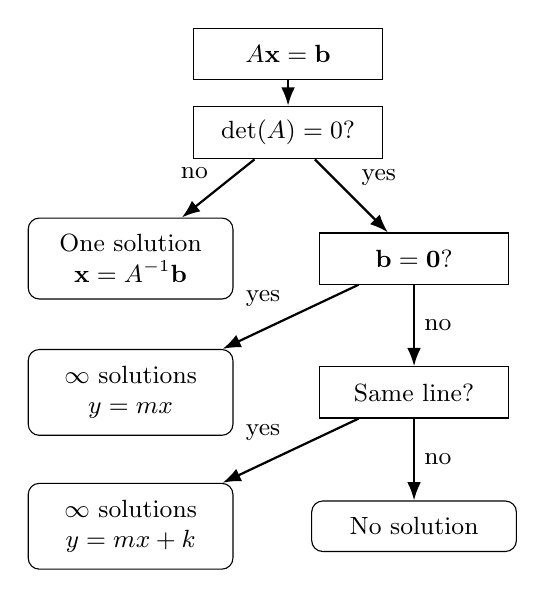
\begin{tikzpicture}[
    every node/.style={font=\small,align=center},
    decision/.style={
        rectangle,draw,
        minimum width=2.4cm,
        minimum height=0.65cm,
        inner sep=5pt
    },
    result/.style={
        rectangle,draw,rounded corners,
        minimum width=2.6cm,
        inner sep=6pt
    },
    line/.style={-Latex,thick}
]

\node[decision] (start) at (0,0)
    {$A\mathbf{x}=\mathbf{b}$};

\node[decision] (det) at (0,-1.0)
    {$\det(A)=0$?};

\node[result] (unique) at (-2,-2.6)
    {One solution\\
     $\mathbf{x}=A^{-1}\mathbf{b}$};

\node[decision] (zero) at (1.6,-2.6)
    {$\mathbf{b}=\mathbf{0}$?};

\node[result] (homogeneous) at (-2,-4.3)
    {$\infty$ solutions\\
     $y=mx$};

\node[decision] (same) at (1.6,-4.3)
    {Same line?};

\node[result] (infinite) at (-2,-6)
    {$\infty$ solutions\\
     $y=mx+k$};

\node[result] (none) at (1.6,-6)
    {No solution};

\draw[line] (start) -- (det);

\draw[line] (det) --
    node[above left] {no} (unique);
\draw[line] (det) --
    node[above right] {yes} (zero);

\draw[line] (zero) --
    node[above left] {yes} (homogeneous);
\draw[line] (zero) --
    node[right] {no} (same);

\draw[line] (same) --
    node[above left] {yes} (infinite);
\draw[line] (same) --
    node[right] {no} (none);
\end{tikzpicture}
\end{center}



\end{document}